\subsection{Ejercicio 12}
\graphicspath{ {img/12} }

Los sitios web seleccionados fueron:
\begin{itemize}
    \item \url{www.wikipedia.org}
    \item \url{https://elpais.com/}
\end{itemize}

\subsubsection{Cookies almacenadas}

\begin{figure}[H]
    \centering
    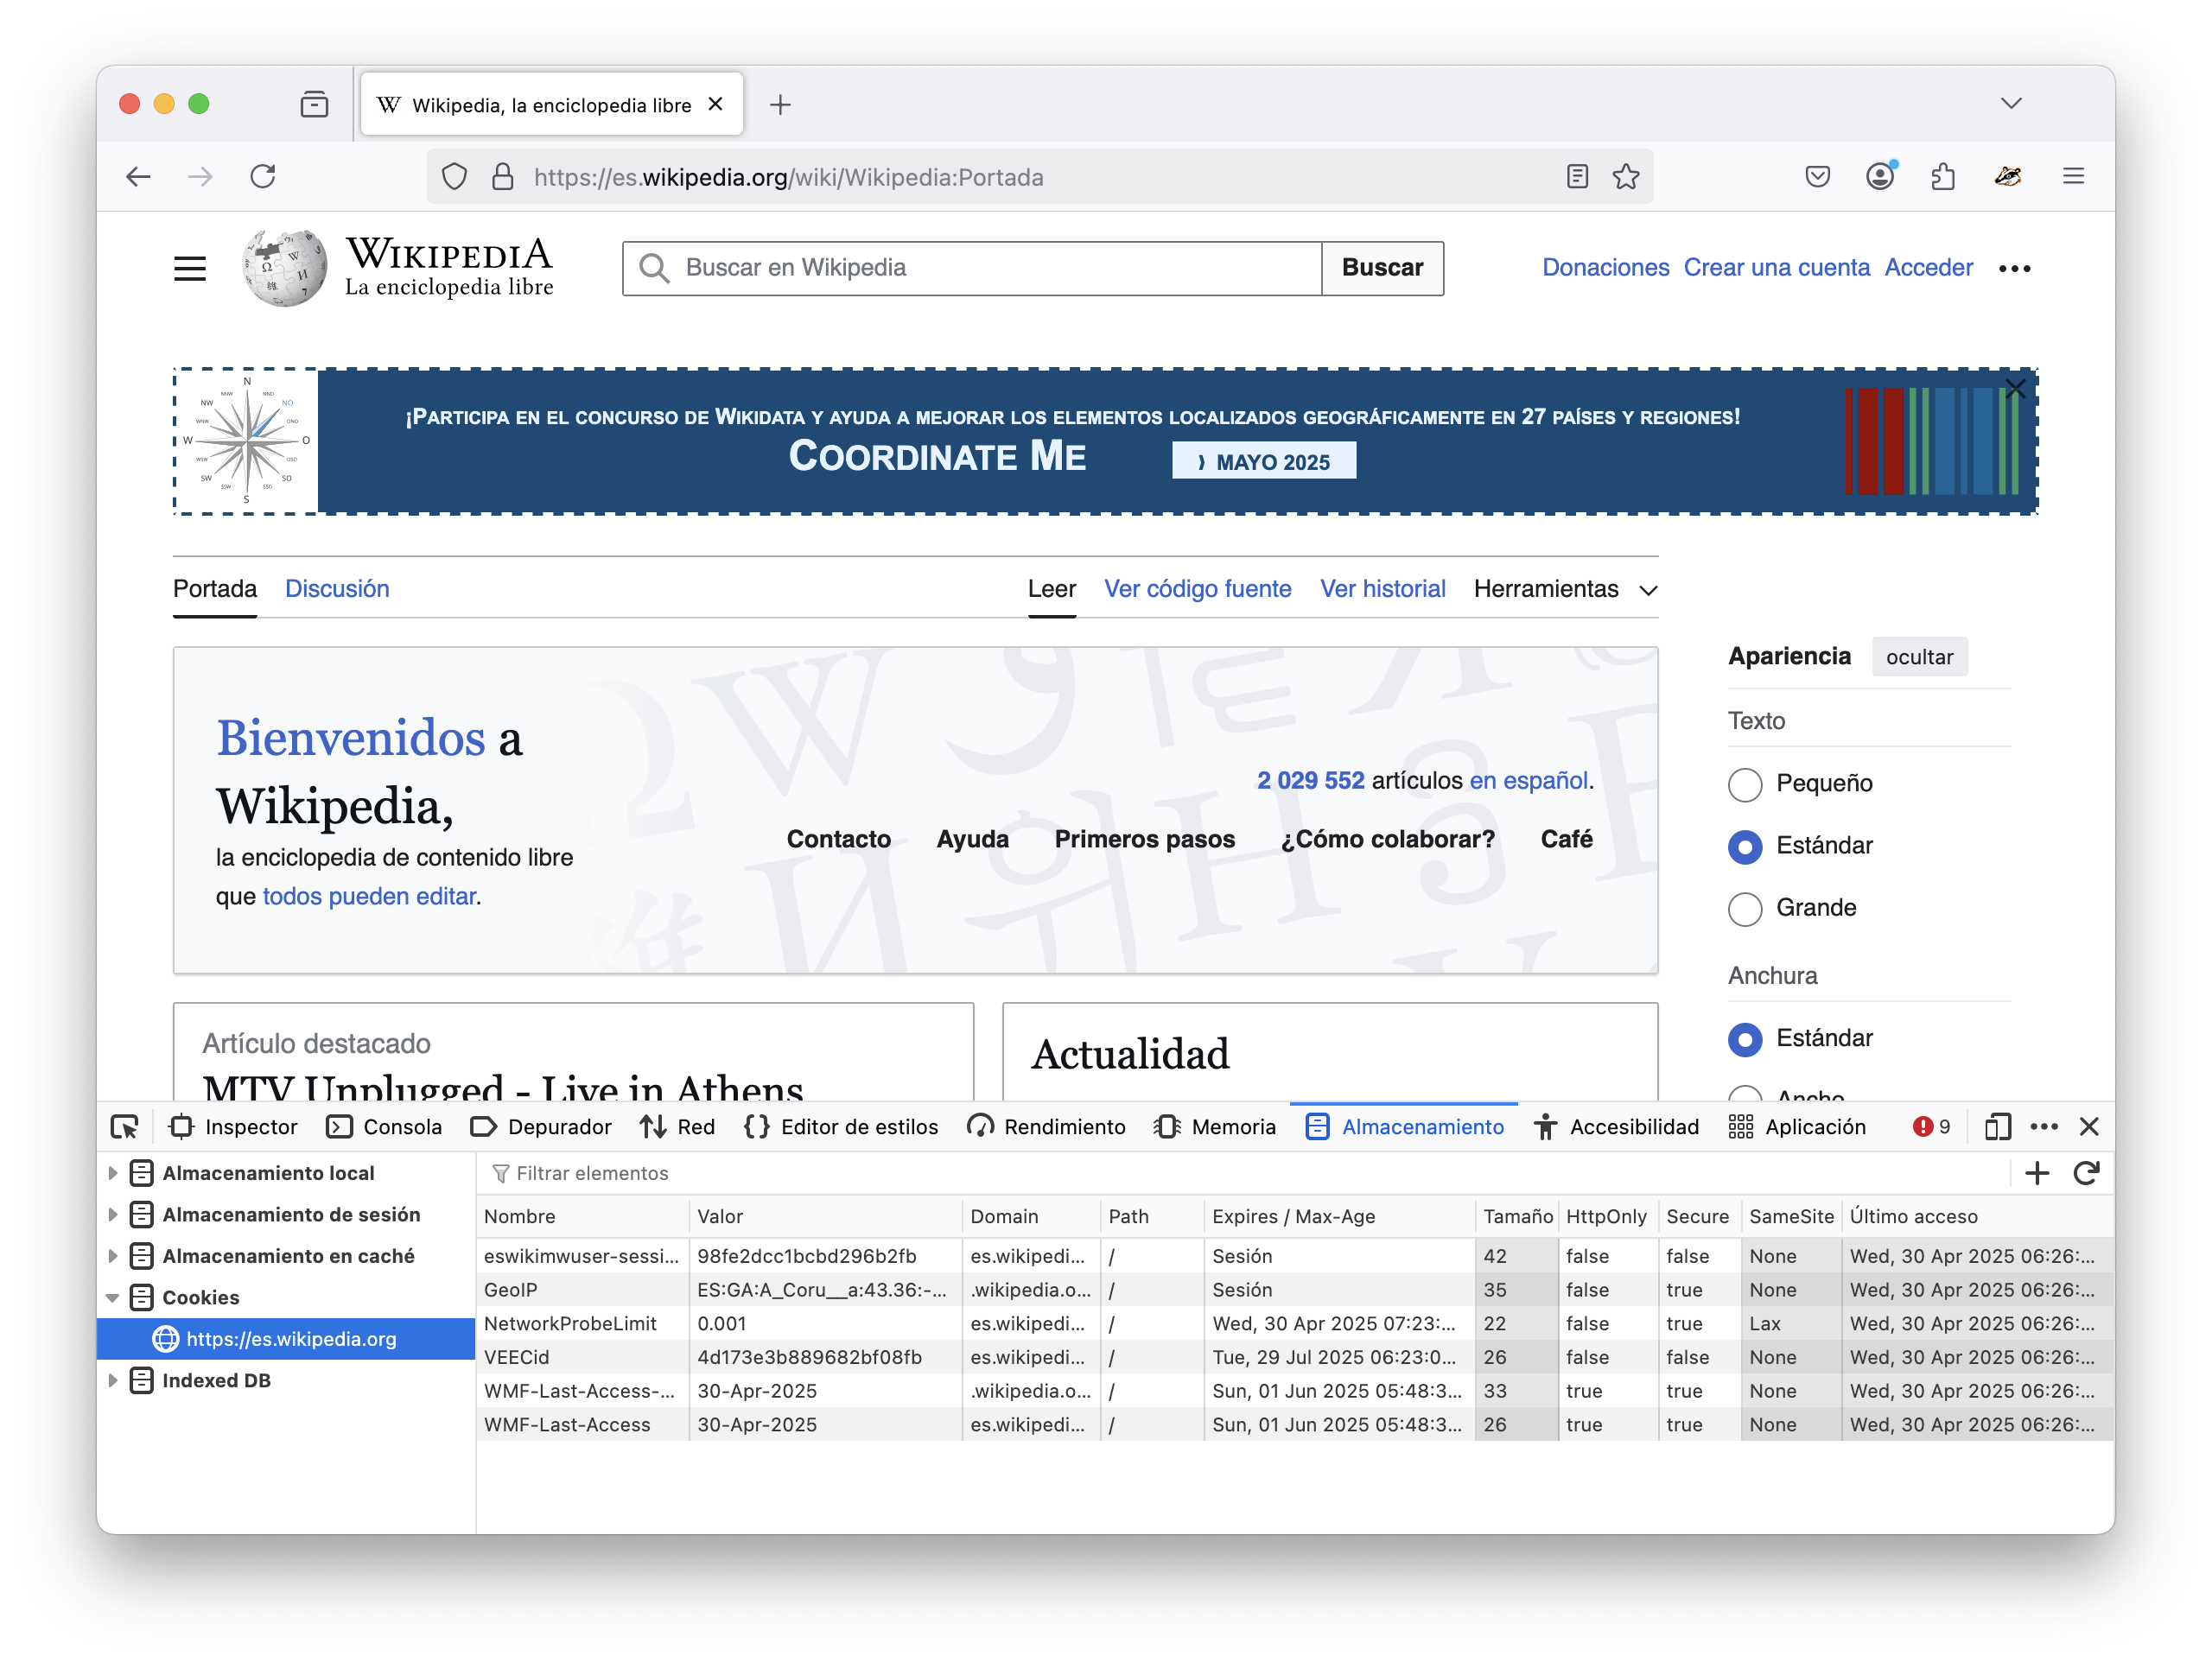
\includegraphics[width=0.9\textwidth]{cookies_wiki.png}
    \caption{Cookies almacenadas por Wikipedia}
    \label{fig:cookies_wiki}
\end{figure}

El primer sitio web seleccionado es la Wikipedia. Para poder ver cuántas cookies se almacenan y cuáles son debemos inspeccionar la página. En la figura \ref{fig:cookies_wiki} podemos ver cuáles son las cookies que se almacenan en el sitio web. Las 6 cookies almacenadas son: \texttt{eswikiwmuser-sessionId}, \texttt{GeoIP}, \texttt{NetworkProbeLimit}, \texttt{WMF-Last-Access} (parece duplicada con distinto valor o ámbito de acceso) y \texttt{centralnotice\_fundraising}.

Seleccionamos la cookie \texttt{GeoIP} para su análisis. Esta cookie contiene información sobre la localización del usuario (por ejemplo, país y región), y presenta los siguientes parámetros:

\begin{itemize}
    \item \texttt{Expires (Sesión)}: se elimina al cerrar el navegador, lo que limita su persistencia.
    \item \texttt{HttpOnly (false)}: puede ser accedida mediante scripts JavaScript, lo cual implica un riesgo si hubiera un ataque de tipo XSS.
    \item \texttt{Secure (false)}: puede transmitirse incluso si la conexión no es segura, aunque Wikipedia usa HTTPS por defecto.
    \item \texttt{SameSite (None)}: permite que esta cookie se envíe en peticiones entre sitios (cross-site), lo cual es potencialmente más vulnerable a ataques CSRF si no se combina con otras medidas.
\end{itemize}

Aunque la cookie no contiene datos especialmente sensibles, la combinación de \\\texttt{Secure=false}, \texttt{HttpOnly=false} y \texttt{SameSite=None} la hace más vulnerable que otras cookies más restringidas. Sin embargo, dado que Wikipedia utiliza HTTPS obligatorio y no utiliza cookies de sesión crítica para usuarios no registrados, el riesgo real es bajo.

\begin{figure}[H]
    \centering
    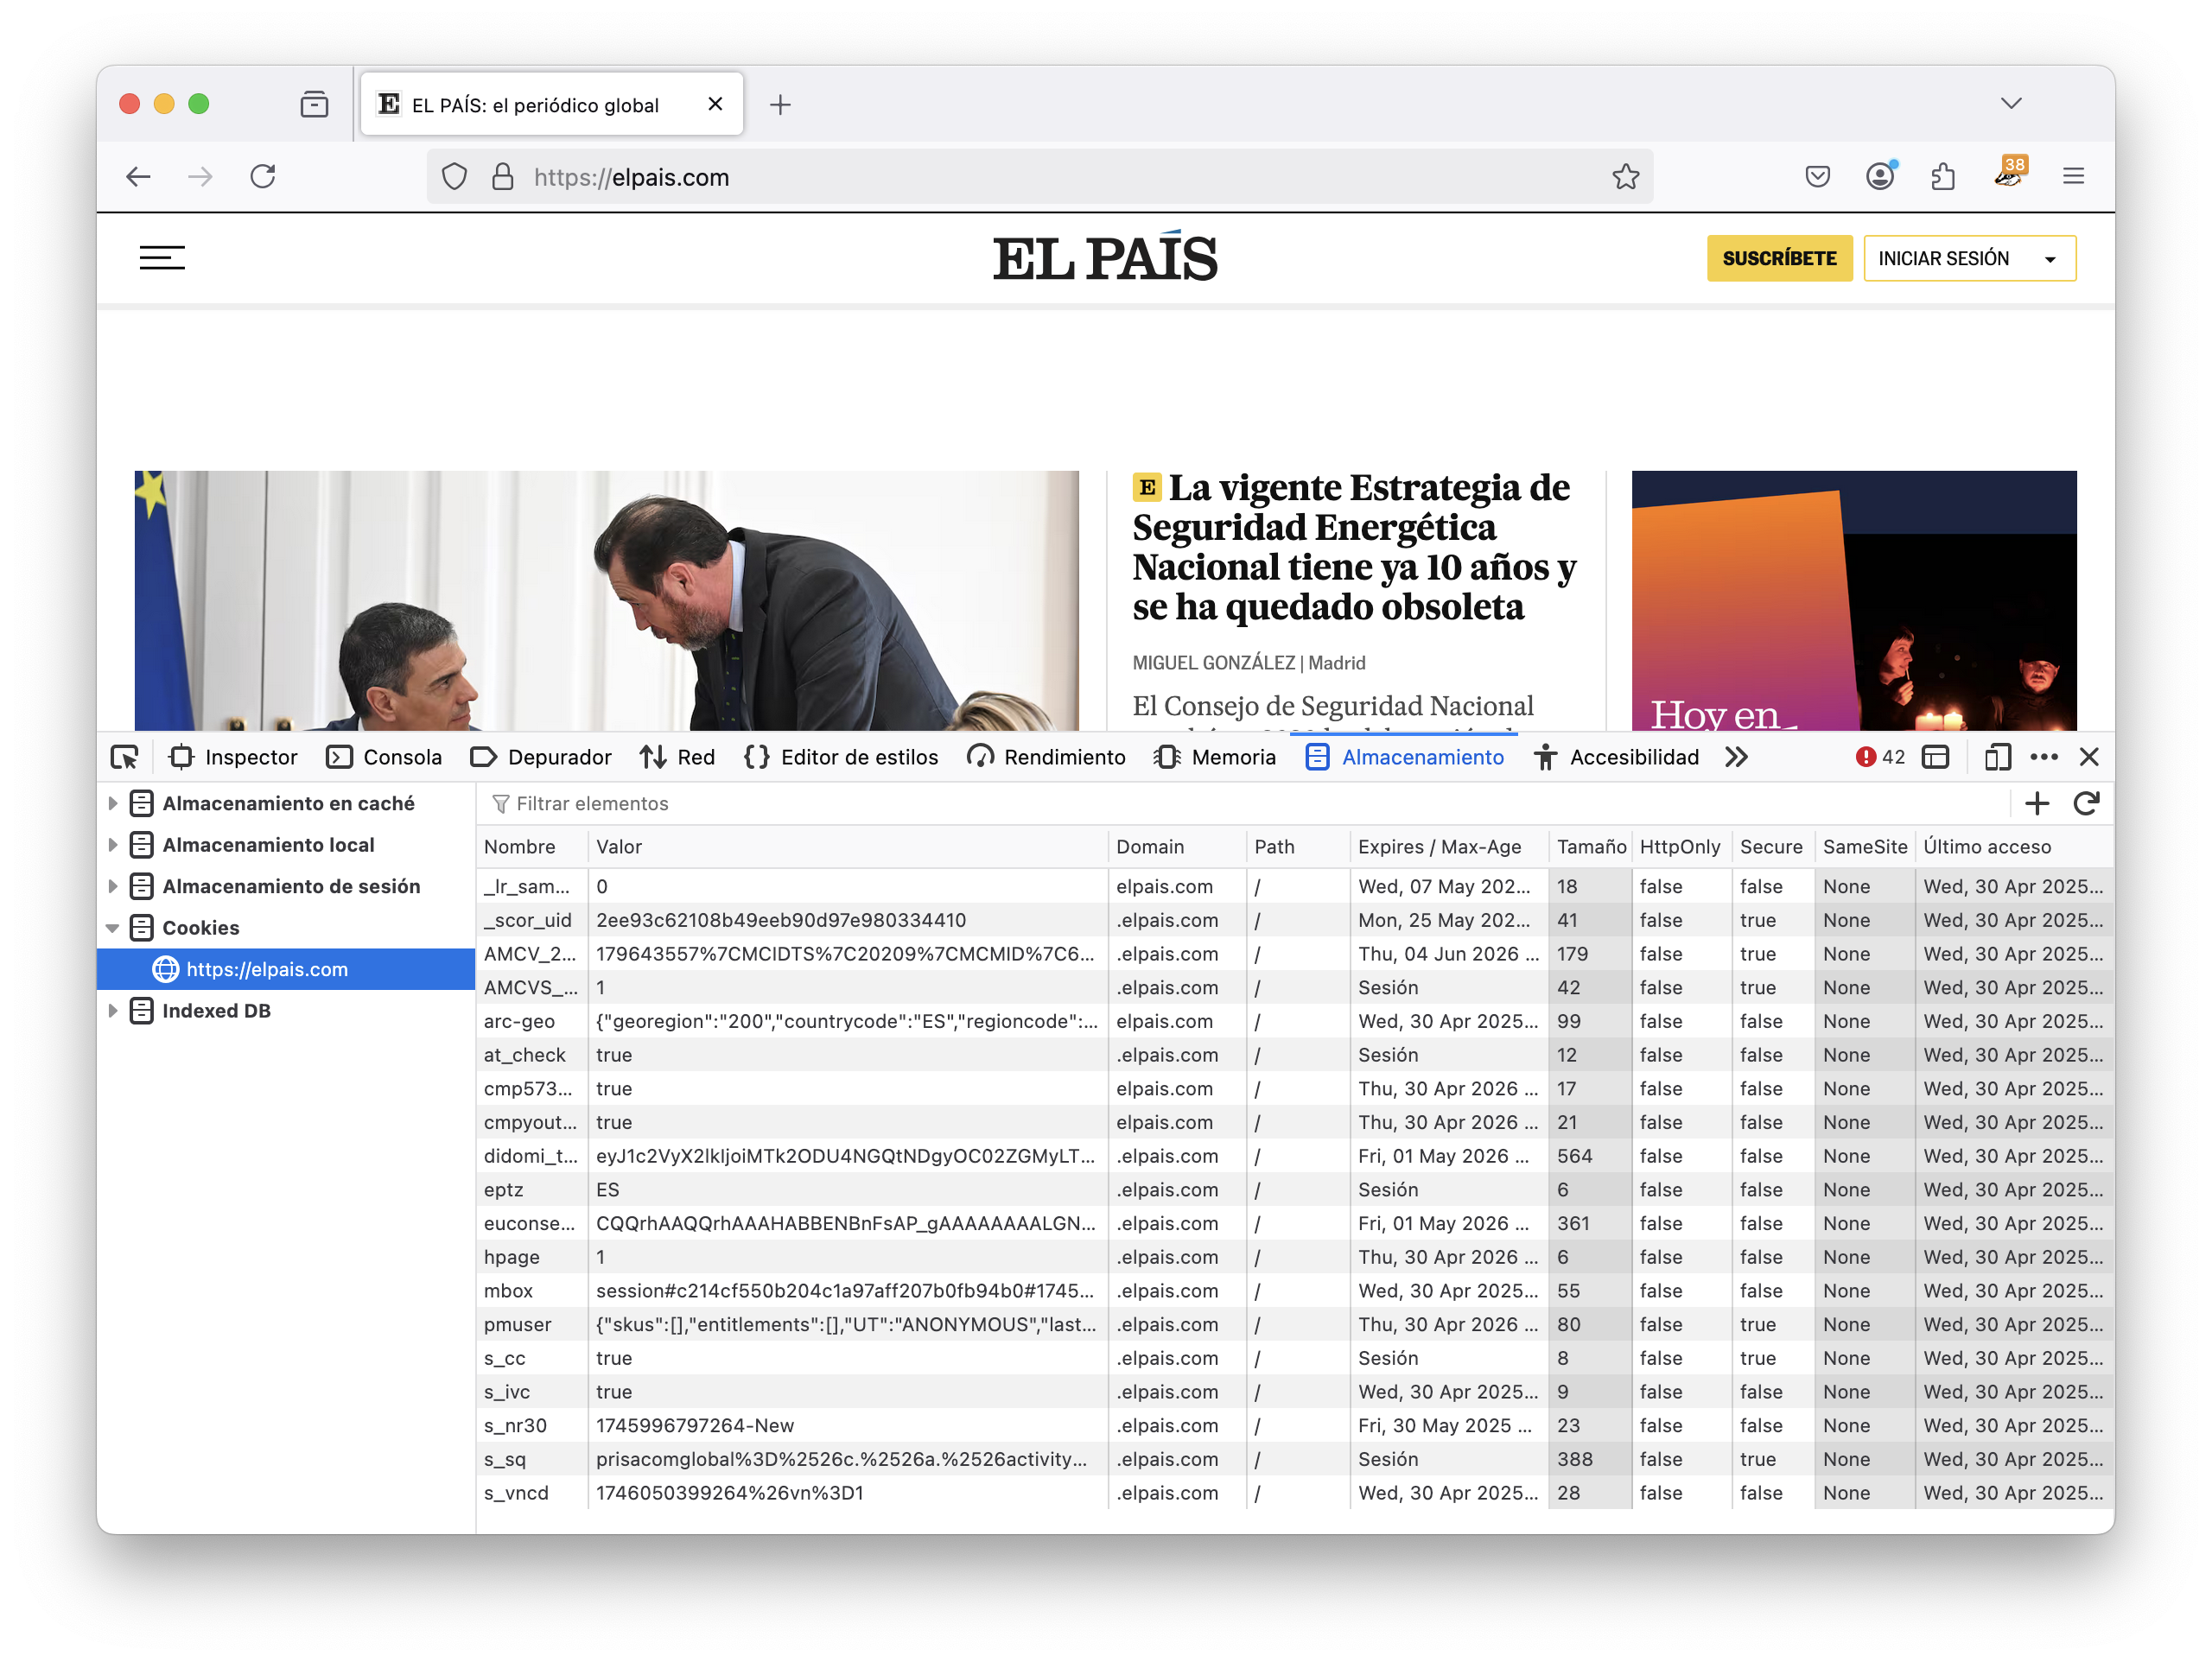
\includegraphics[width=\textwidth]{cookies_pais.png}
    \caption{Cookies almacenadas por El Pais}
    \label{fig:cookies_pais}
\end{figure}

El segundo sitio web seleccionado es El País. Tal y como hicimos con el dominio anterior, debemos inspeccionar la página. En la figura \ref{fig:cookies_pais} podemos ver cuáles son las cookies que se almacenan en el sitio web. Se almacenan un total de 20 cookies distintas, todas ellas asociadas al mismo dominio, elpais.com.

Seleccionamos la cookie \texttt{AMCVS\_} para su análisis. Esta cookie está relacionada con Adobe Analytics y se utiliza para identificar sesiones de usuario. Presenta los siguientes parámetros:

\begin{itemize}
    \item \texttt{Expires (Sesión)}: se elimina al cerrar el navegador, lo que limita su persistencia.
    \item \texttt{HttpOnly (false)}: puede ser accedida mediante scripts JavaScript, lo cual implica un riesgo si hubiera un ataque de tipo XSS.
    \item \texttt{Secure (true)}: solo se transmite a través de conexiones HTTPS, lo cual mejora su seguridad.
    \item \texttt{SameSite (None)}: permite que esta cookie se envíe en peticiones entre sitios (cross-site), lo cual es potencialmente más vulnerable a ataques CSRF si no se combina con otras medidas.
\end{itemize}

Aunque la cookie no contiene información directamente sensible, el hecho de que sea accesible desde JavaScript (\texttt{HttpOnly=false}) y pueda ser enviada entre sitios \\(\texttt{SameSite=None}) la hace más expuesta a ciertos ataques, especialmente si el sitio web tiene fallos de seguridad no corregidos. No obstante, al estar marcada como Secure, su transmisión está protegida frente a interceptación en redes no cifradas.

\subsubsection{Cookies persistentes y de sesión}

Para determinar si las cookies almacenadas en ambos dominios web, debemos analizar el campo \texttt{Expires/Max-Age}. En función de su persistencia, podemos dividir las cookies en dos grupos: persistentes y de sesión. Las cookies persistentes tienen fecha de expiración futura, lo que significa que se guardan incluso después de cerrar el navegador. Al contrario que las anteriores, las cookies de sesión se eliminan al cerrar el navegador. Se identifican fácilmente, pues en el campo mencionado toman el valor \texttt{Sesión}.

En el caso de la Wikipedia, las cookies persistentes son: \texttt{NetworkProbeLimit} (expira el 30 de abril de 2025), \texttt{WMF-Last-Access 1} (expira el 29 de julio de 2025), \texttt{WMF-Last-Access 2} (expira el 1 de junio de 2025) y \texttt{centralnotice\_fundraising} (expira el 1 de junio de 2025). Las cookies que se borrarán al cerrar el navegador son: \texttt{eswikiwmuser-sessionId} y \texttt{GeoIP}.

En el caso de El País, de entre sus 20 cookies distintas, las que se borrarán al cerrar el navegador son: \texttt{AMCVS\_}, \texttt{arc-check}, \texttt{ept2} y \texttt{sessionfc}. Las 16 cookies restantes son persistentes, ya que muestran fechas de caducidad. El rango de expiración de las cookies persistentes en elpais.com va desde el 30 de abril de 2025 hasta el 4 de agosto de 2026, lo que indica que algunas cookies están pensadas para mantenerse activas durante más de un año, especialmente aquellas vinculadas a analítica o personalización del usuario.

\subsubsection{Cookies de terceros}

Como se ve en la figura \ref{fig:cookies_wiki}, en el momento de la visita a Wikipedia, no se almacenaron cookies de terceros. Todas las cookies visibles pertenecen al dominio principal es.wikipedia.org, lo cual es coherente con la política de privacidad de Wikipedia, que no utiliza rastreadores ni servicios publicitarios externos en su página principal.

Por otra parte, como se ve en la figura \ref{fig:cookies_pais}, en el momento de la visita a El País, se observa que todas las cookies están asociadas al dominio elpais.com, por lo que se consideran cookies de primera parte. No obstante, es posible que se carguen cookies de terceros más adelante, si se acepta el uso de publicidad personalizada o se navega más profundamente por el sitio.

\subsubsection{Cookies eliminadas y navegación privada}

Para eliminar todas las cookies de ambos sitios web, debemos hacer click derecho en cualquiera de las cookies que se ven en las figuras \ref{fig:cookies_wiki} y \ref{fig:cookies_pais}, y seleccionamos la opción \texttt{Eliminar todo de 'es.wikipedia.org'} en el caso de Wikipedia y \texttt{Eliminar todo de 'elpais.com'}. Una vez hecho esto, procedimos a acceder a ambas webs en modo navegación privada.

\begin{figure}[H]
    \centering
    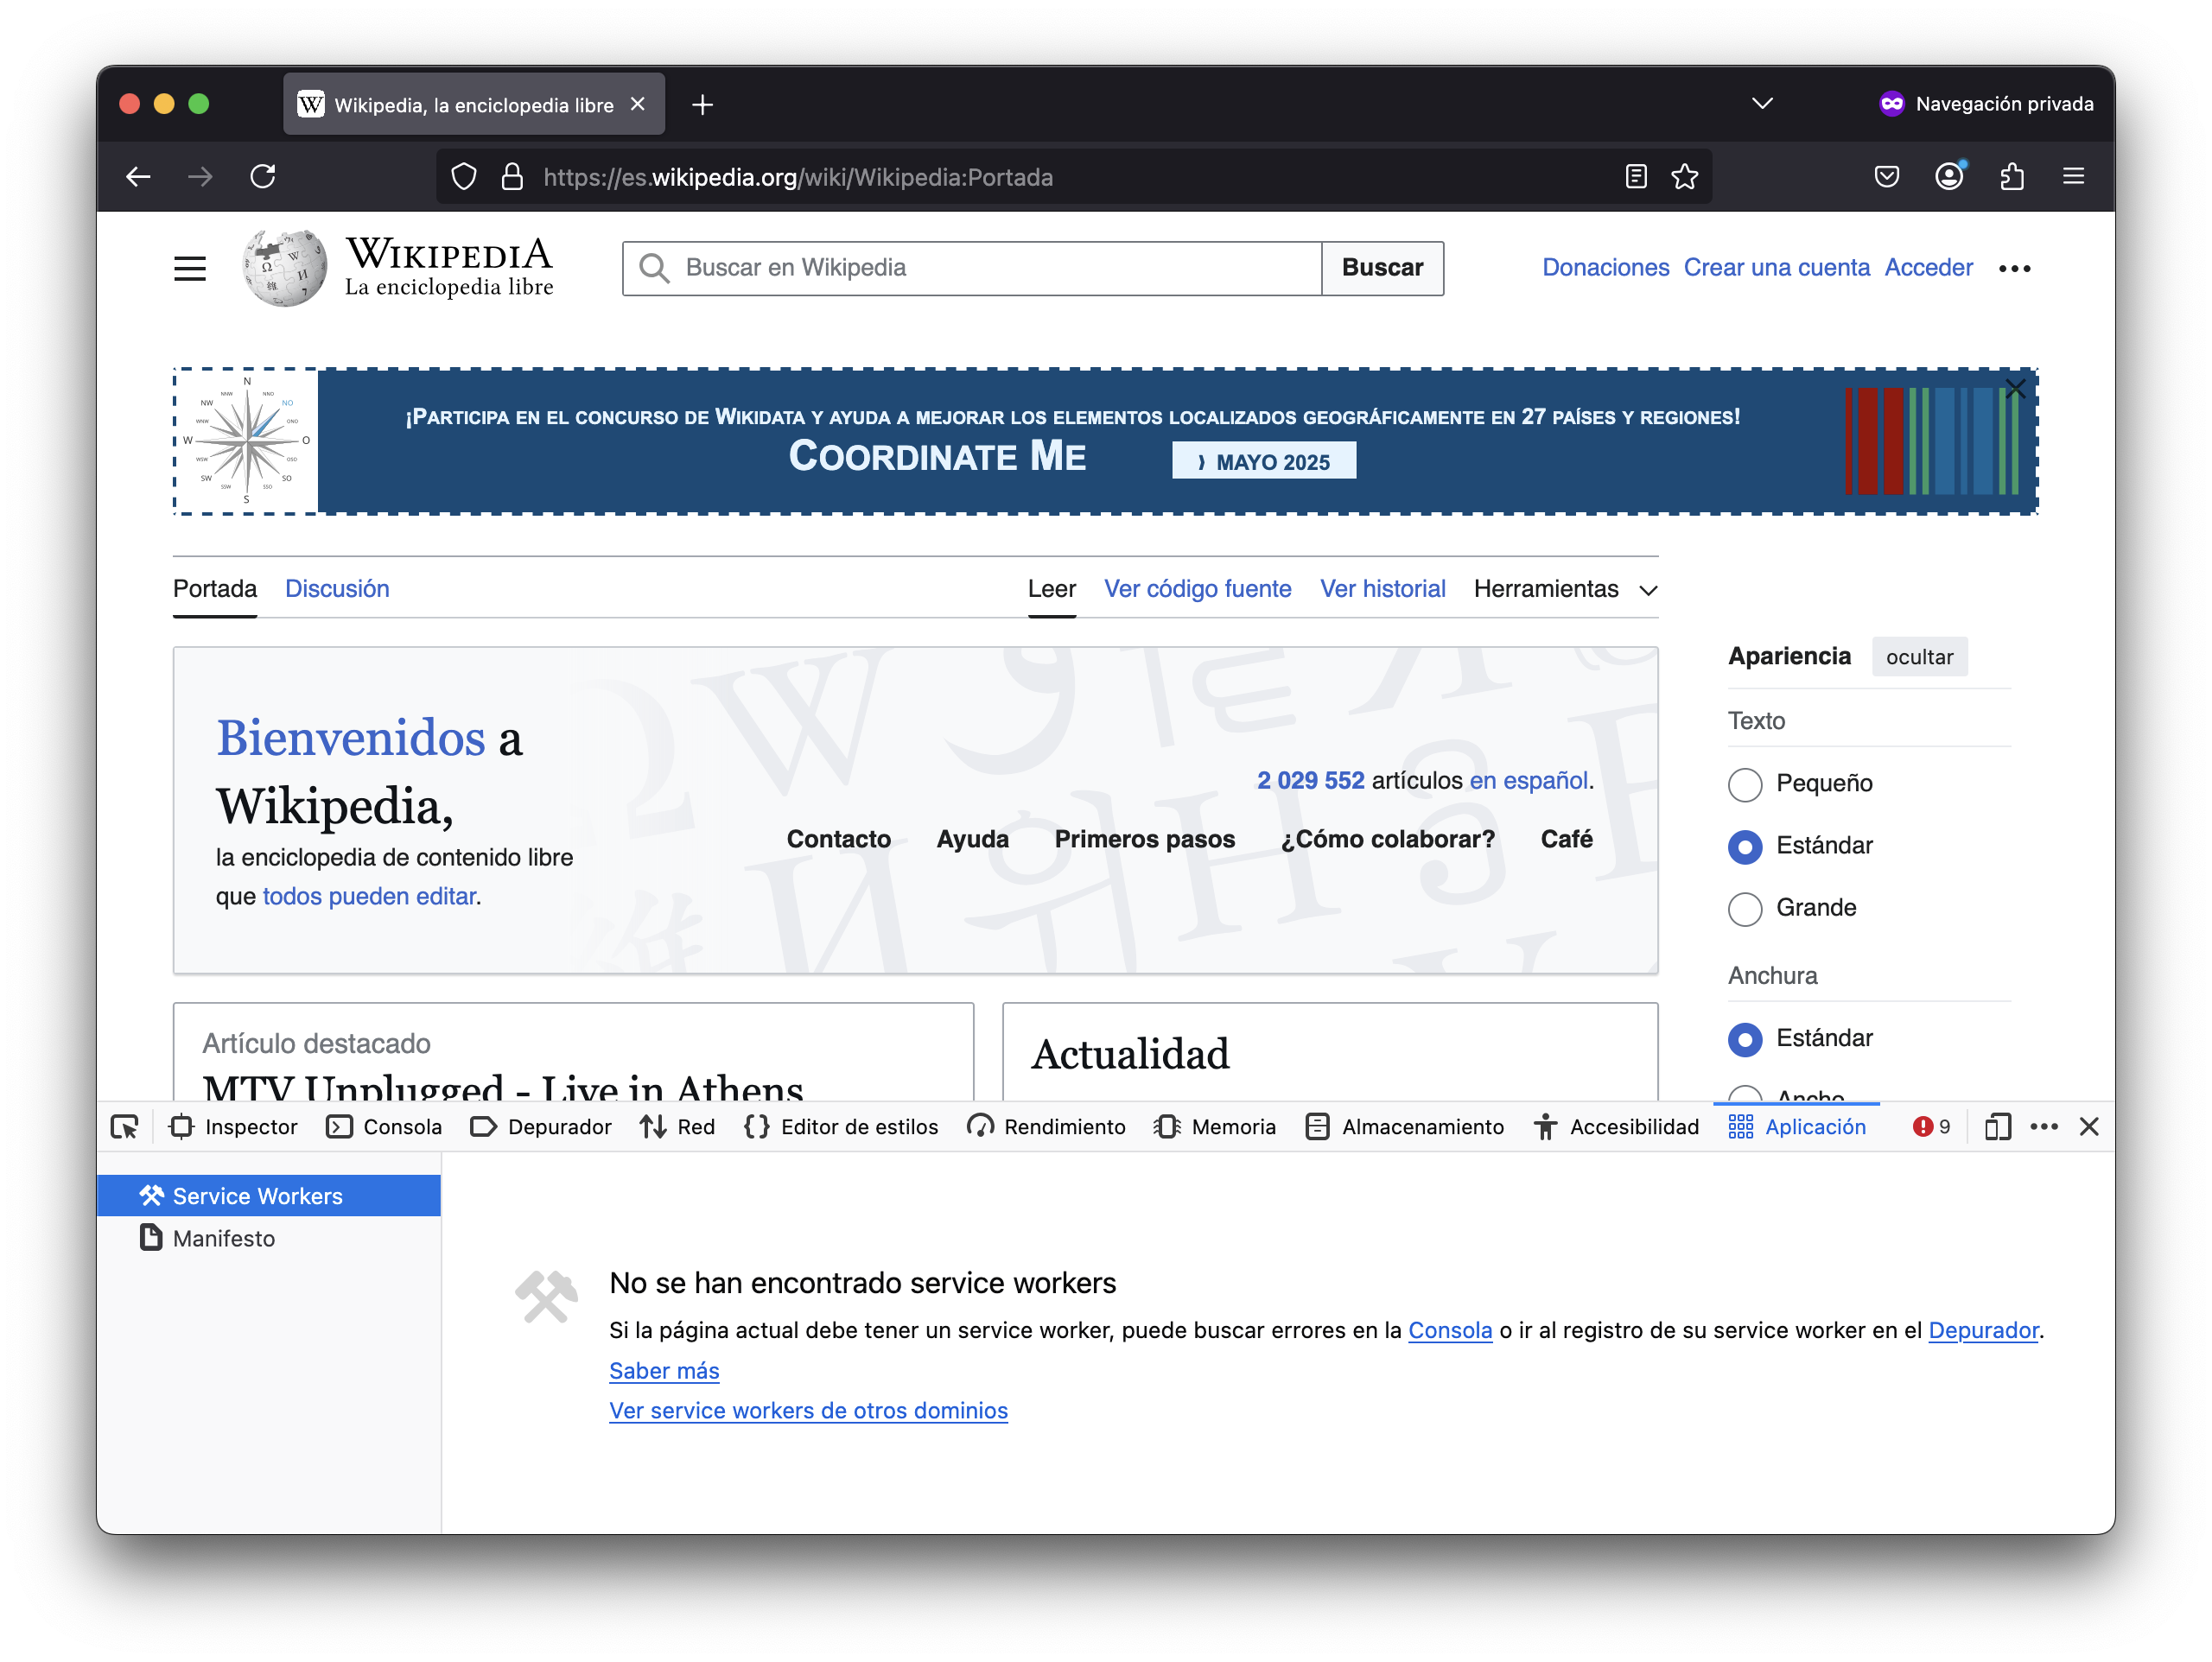
\includegraphics[width=\textwidth]{cookies_wiki_npriv.png}
    \caption{Cookies almacenadas por Wikipedia en navegación privada tras eliminación}
    \label{fig:cookies_wiki_npriv}
\end{figure}

Al eliminar todas las cookies del sitio \url{wikipedia.org}, se borra toda la información previamente almacenada, incluyendo identificadores de sesión, preferencias de idioma o geolocalización (por ejemplo, cookies como GeoIP o WMF-Last-Access). Sin embargo, la navegación por el sitio no se ve afectada, ya que Wikipedia no depende de cookies para su funcionamiento básico, especialmente si el usuario no ha iniciado sesión.

Al acceder a Wikipedia en modo de navegación privada, se comprueba, como se muestra en \ref{fig:cookies_wiki_npriv}, que no se han generado cookies persistentes ni otros datos de almacenamiento, como service workers o bases de datos. Esto es coherente con el comportamiento de Wikipedia, que aplica una política de privacidad estricta: no utiliza rastreadores ni cookies de terceros, y solo crea cookies mínimas y temporales necesarias para aspectos técnicos. Además, al cerrar la ventana privada, cualquier cookie temporal generada durante la sesión se elimina automáticamente, dejando el navegador sin rastro de la actividad.

\begin{figure}[H]
    \centering
    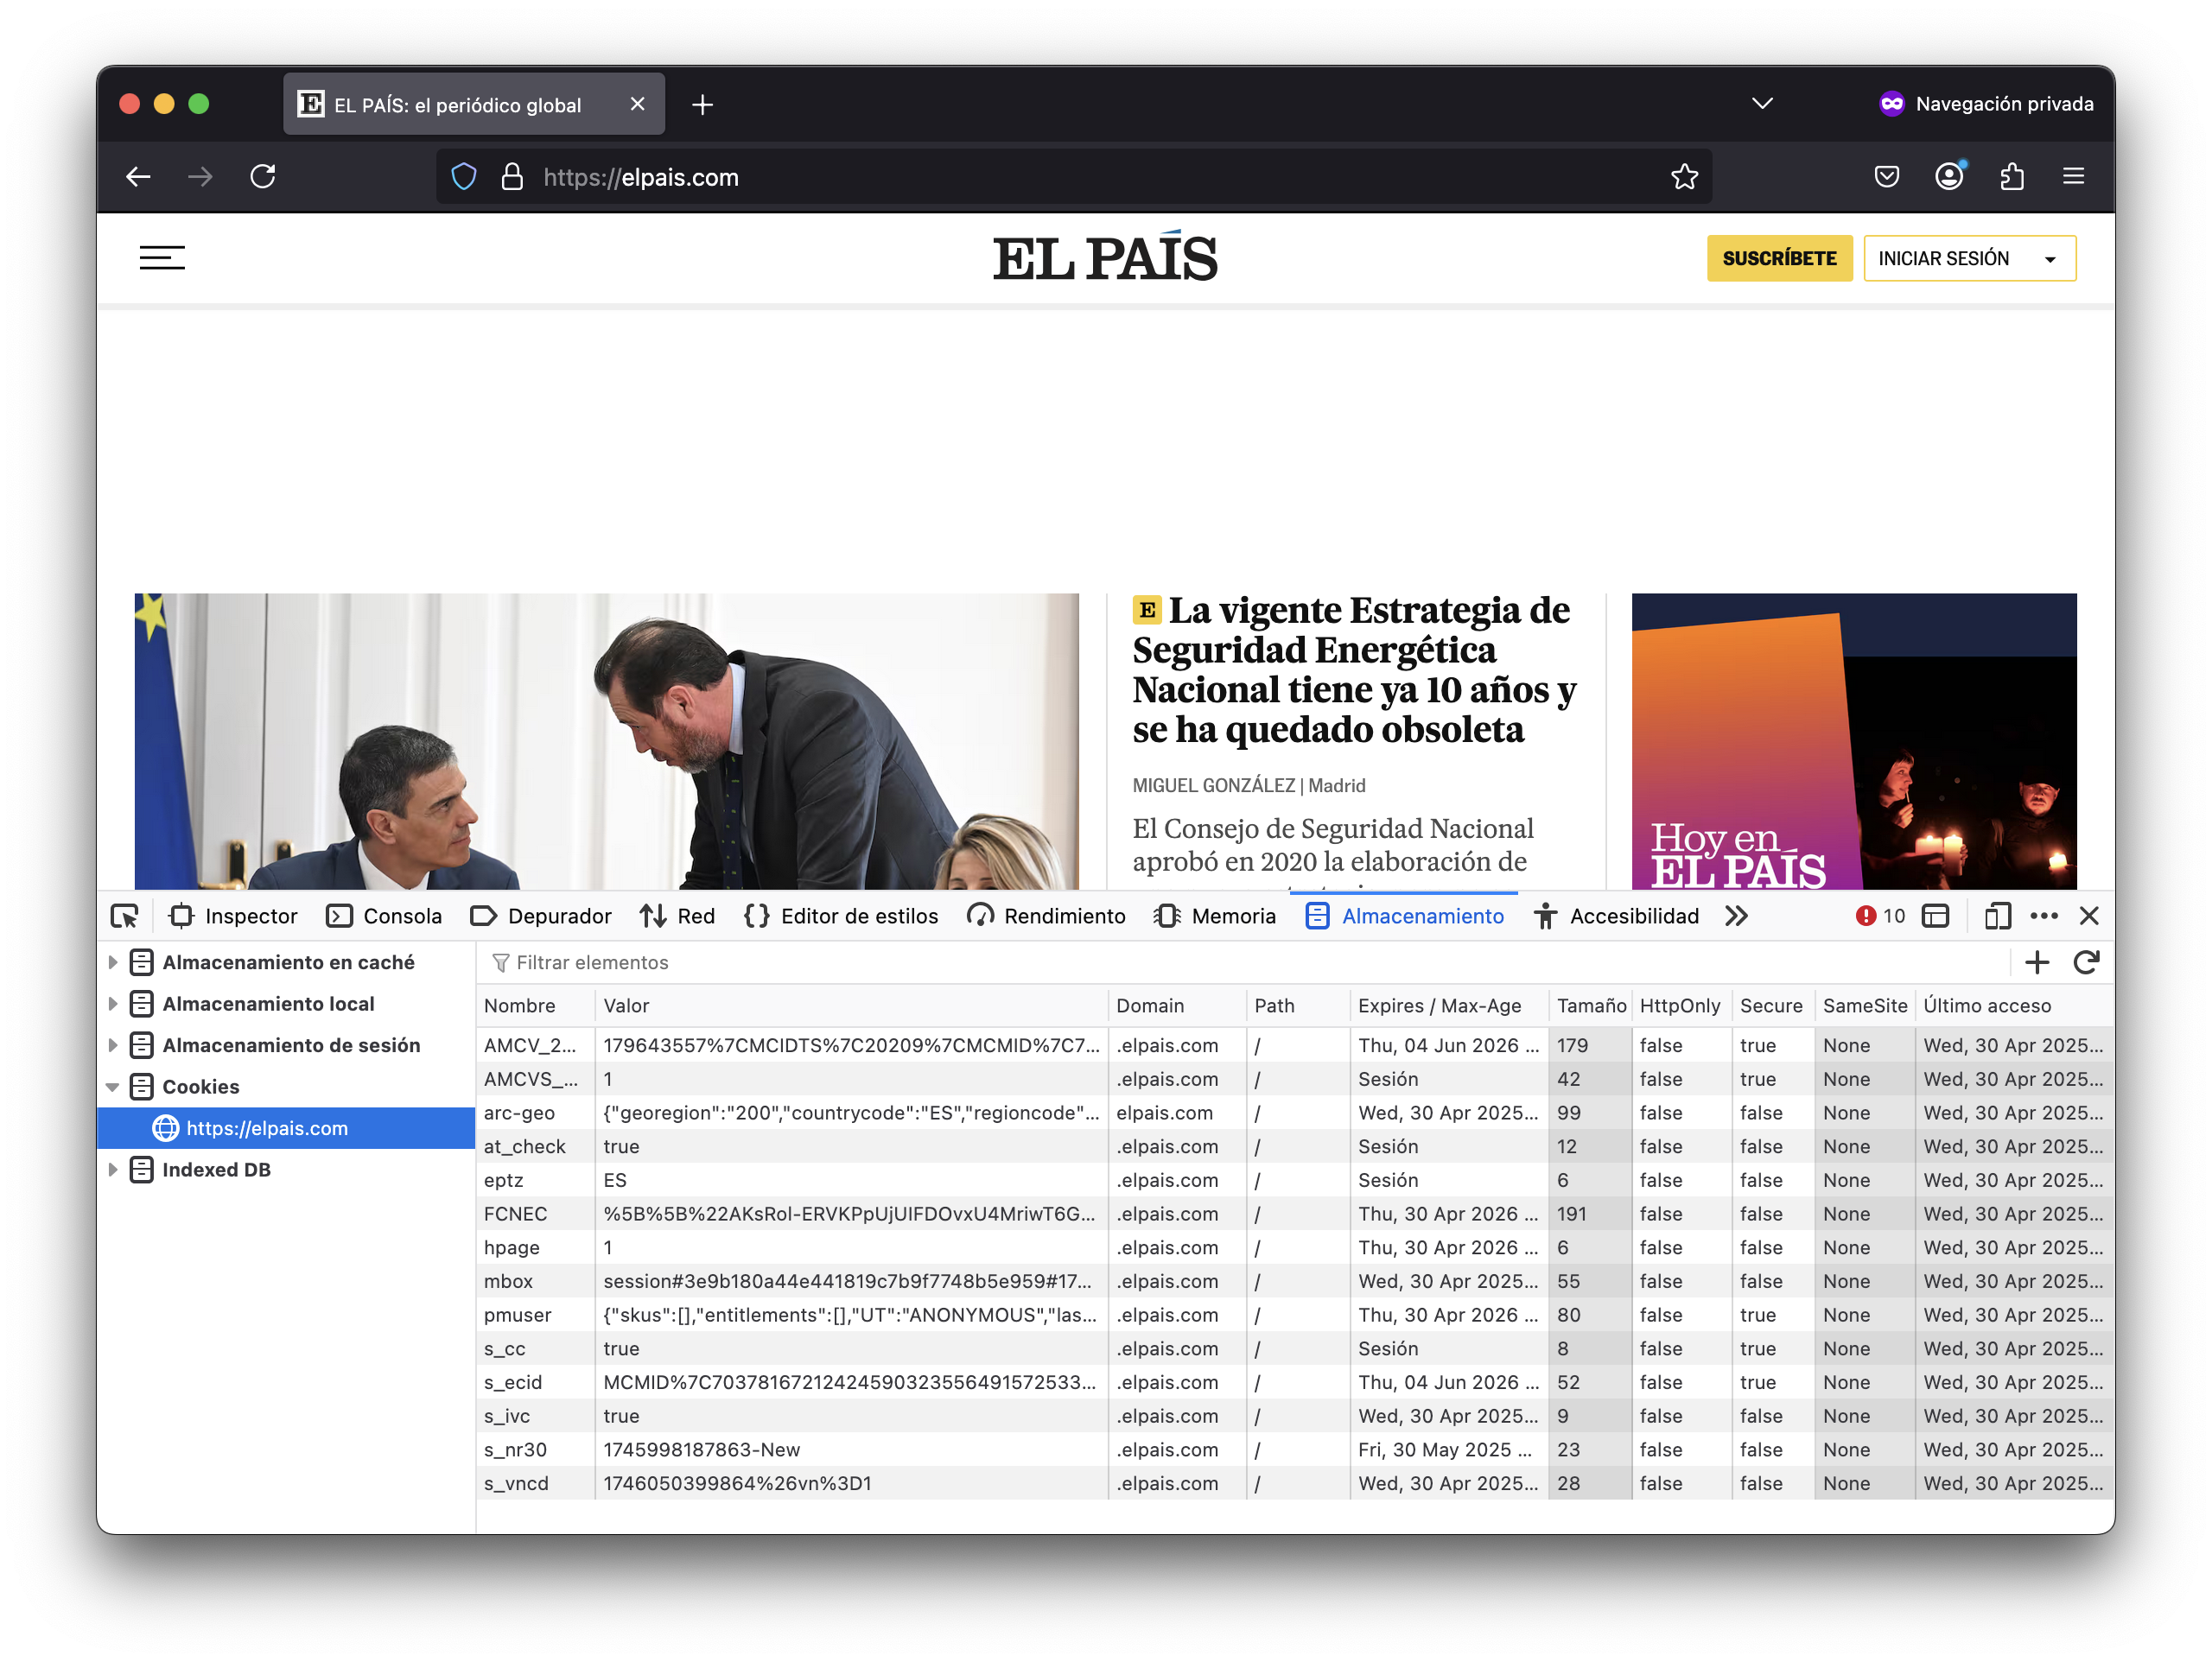
\includegraphics[width=\textwidth]{cookies_pais_npriv.png}
    \caption{Cookies almacenadas en El País en navegación privada tras eliminación}
    \label{fig:cookies_pais_npriv}
\end{figure}

Al eliminar todas las cookies del sitio \url{elpais.com}, se pierde la información relacionada con la sesión, el consentimiento de cookies y otros datos de navegación. Al volver a visitar la página, se muestra nuevamente el aviso de consentimiento, y el sitio crea nuevas cookies mínimas para gestionar la sesión. La navegación no se ve interrumpida, pero se reinicia el seguimiento y es necesario volver a aceptar (o rechazar) las cookies para personalizar la experiencia.

Tras acceder en modo de navegación privada, como se ve en la figura \ref{fig:cookies_pais_npriv}, el sitio vuelve a generar varias cookies, como \texttt{AMCVS\_}, \texttt{arc\_geo}, \texttt{mbox}, \texttt{s\_cc}, entre otras. Esto se debe a que al abrir una ventana privada el navegador empieza con una sesión vacía, es decir, sin ninguna cookie de ningún tipo de las que tenemos en nuestra sesión habitual. Estas cookies que se añaden permiten el funcionamiento del sitio y de ciertos servicios, pero todas ellas, independientemente de si son temporales o no, se borrarán automáticamente al cerrar el sitio web.
